\section*{Questão 2}

Um robô pode se mover pelos quadrados da figura abaixo. A cada unidade de tempo (minuto, por exemplo), o robô tenta se mover para um dos quadrados adjacentes ao que ocupa e escolhe uma dentre as possíveis ações: (a) mover para Norte; (b) mover para Sul; (c) mover para Leste; (d) mover para Oeste. O robô não consegue enxergar a sua volta, então escolhe aleatoriamente uma dentre as 4 ações possíveis para só então fazer um movimento. Caso o robô tenha escolhido se mover na direção de um dos quadrados em rosa (os com tijolinhos na Figura 1) ou para fora do ambiente, ele colide com a parede e permanece na mesma posição até a nova tentativa.

\begin{figure}[H]
    \centering
    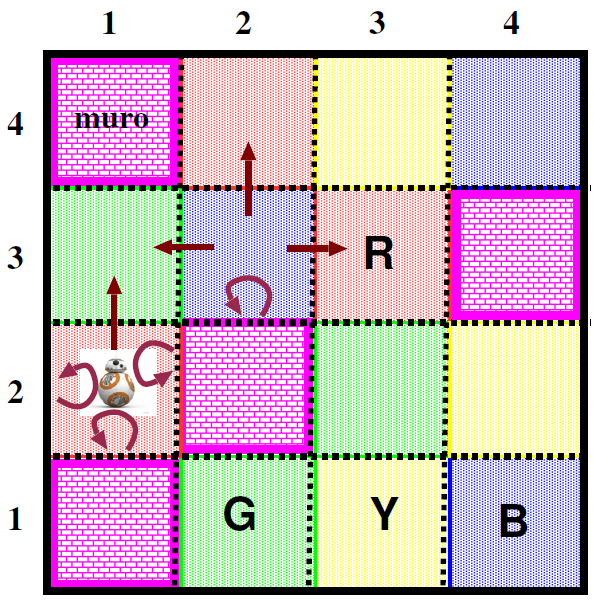
\includegraphics[width=8cm]{fig/enunciado_q2.png}
    \caption{Robô andando por um ambiente}
\end{figure}

\begin{enumerate}
    \item \textbf{Construa a cadeia de Markov que representa o movimento do robô pelo ambiente, e mostre a matriz de transição de estados do sistema. Para facilitar a correção, indique claramente quais os estados do sistema e exemplifique indicando as probabilidades de transição para um movimento.}
    
    Considerando que a probabilidade de o robô escolher uma das ações possíveis é igual para todas as ações, a Cadeia de Markov que representa o movimento do robô no ambiente é dada na Figura \ref{fig:cadeia_markov_redundante}.
    
    \begin{figure}[H]
        \centering
        \begin{tikzpicture}[->, >=stealth, node distance=2.5cm, auto]
        
        % Define nodes with inverted y-axis and two-digit labels
        \node[state] (11) at (0,0) {(1,1)};
        \node[state] (12) [right=of 11] {(1,2)};
        \node[state] (13) [right=of 12] {(1,3)};
        \node[state] (14) [right=of 13] {(1,4)};
            
        \node[state] (21) [above=of 11] {(2,1)};
        \node[state] (22) [above=of 12] {(2,2)};
        \node[state] (23) [above=of 13] {(2,3)};
        \node[state] (24) [above=of 14] {(2,4)};
            
        \node[state] (31) [above=of 21] {(3,1)};
        \node[state] (32) [above=of 22] {(3,2)};
        \node[state] (33) [above=of 23] {(3,3)};
        \node[state] (34) [above=of 24] {(3,4)};
            
        \node[state] (41) [above=of 31] {(4,1)};
        \node[state] (42) [above=of 32] {(4,2)};
        \node[state] (43) [above=of 33] {(4,3)};
        \node[state] (44) [above=of 34] {(4,4)};


        % Transitions for node (1,2)
        \path (12) edge [loop below] node {0.25} (12) % Loop because moving south hits the bottom border
                edge [loop left] node {0.25} (12) % Loop because moving west hits the wall at (1,1)
                edge [loop above] node {0.25} (12) % Loop because moving north hits the wall at (2,2)
                edge[bend left] node[above] {0.25} (13);

        % Transitions for node (1,3)
        \path (13) edge [loop below] node {0.25} (13) % Loop because moving south hits the bottom border
                edge[bend left] node[below] {0.25} (12)
                edge[bend left] node[above] {0.25} (14)
                edge[bend left] node[above] {0.25} (23);

        % Transitions for node (1,4)
        \path (14) edge [loop right] node {0.25} (14) % Loop because moving east hits the right border
                edge [loop below] node {0.25} (14) % Loop because moving south hits the bottom border
                edge[bend left] node[below] {0.25} (13)
                edge[bend left] node[right] {0.25} (24);

        % Transitions for node (2,1)
        \path (21) edge [loop left] node {0.25} (21) % Loop because moving west hits the left border
                edge[loop below] node {0.25} (21) % Loop because moving south hits the wall at (1,1)
                edge[loop right] node {0.25} (21) % Loop because moving east hits the wall at (1,2)
                edge[bend left] node[above] {0.25} (31);

        % Transitions for node (2,3)
        \path (23) edge[bend left] node[below] {0.25} (13)
                edge[loop left] node {0.25} (23) % Loop because moving west hits the wall at (2,2)
                edge[bend left] node[above] {0.25} (24)
                edge[bend left] node[right] {0.25} (33);

        % Transitions for node (2,4)
        \path (24) edge [loop right] node {0.25} (24) % Loop because moving east hits the right border
                edge[bend left] node[below] {0.25} (14)
                edge[bend left] node[below] {0.25} (23)
                edge[loop above] node {0.25} (24); % Loop because moving north hits the wall at (3,4)

        % Transitions for node (3,1)
        \path (31) edge [loop left] node {0.25} (31) % Loop because moving west hits the left border
                edge[bend left] node[below] {0.25} (21)
                edge[bend left] node[above] {0.25} (32)
                edge[loop above] node {0.25} (31); % Loop because moving north hits the wall at (4,1)

        % Transitions for node (3,2)
        \path (32) edge[loop below] node {0.25} (32) % Loop because moving south hits the wall at (2,2)
                edge[bend left] node[below] {0.25} (31)
                edge[bend left] node[above] {0.25} (33)
                edge[bend left] node[right] {0.25} (42);

        % Transitions for node (3,3)
        \path (33) edge[bend left] node[below] {0.25} (23)
                edge[bend left] node[below] {0.25} (32)
                edge[loop right] node {0.25} (33) % Loop because moving east hits the wall at (3,4)
                edge[bend left] node[right] {0.25} (43);

        % Transitions for node (4,2)
        \path (42) edge [loop above] node {0.25} (42) % Loop because moving north hits the top border
                edge[bend left] node[below] {0.25} (32)
                edge[loop left] node {0.25} (42) % Loop because moving west hits the wall at (4,1)
                edge[bend left] node[above] {0.25} (43);

        % Transitions for node (4,3)
        \path (43) edge [loop above] node {0.25} (43) % Loop because moving north hits the top border
                edge[bend left] node[below] {0.25} (33)
                edge[bend left] node[below] {0.25} (42)
                edge[bend left] node[above] {0.25} (44);

        % Transitions for node (4,4)
        \path (44) edge [loop right] node {0.25} (44) % Loop because moving east hits the right border
                edge [loop above] node {0.25} (44) % Loop because moving north hits the top border
                edge[loop below] node {0.25} (44) % Loop because moving south hits the wall at (3,4)
                edge[bend left] node[below] {0.25} (43);
        
        \end{tikzpicture}
        \caption{Cadeia de Markov representando o movimento do robô no ambiente.}
        \label{fig:cadeia_markov_redundante}
        \end{figure}

Simplificando as transições redundantes nos estados que possuem mais de uma transição retornando para ele mesmo, a Cadeia de Markov que representa o movimento do robô no ambiente sem redundâncias é dada na Figura \ref{fig:cadeia_markov}.

        \begin{figure}[H]
            \centering
            \begin{tikzpicture}[->, >=stealth, node distance=2.5cm, auto]
            
            % Define nodes with inverted y-axis and two-digit labels
            \node[state] (11) at (0,0) {(1,1)};
            \node[state] (12) [right=of 11] {(1,2)};
            \node[state] (13) [right=of 12] {(1,3)};
            \node[state] (14) [right=of 13] {(1,4)};
                
            \node[state] (21) [above=of 11] {(2,1)};
            \node[state] (22) [above=of 12] {(2,2)};
            \node[state] (23) [above=of 13] {(2,3)};
            \node[state] (24) [above=of 14] {(2,4)};
                
            \node[state] (31) [above=of 21] {(3,1)};
            \node[state] (32) [above=of 22] {(3,2)};
            \node[state] (33) [above=of 23] {(3,3)};
            \node[state] (34) [above=of 24] {(3,4)};
                
            \node[state] (41) [above=of 31] {(4,1)};
            \node[state] (42) [above=of 32] {(4,2)};
            \node[state] (43) [above=of 33] {(4,3)};
            \node[state] (44) [above=of 34] {(4,4)};
    
    
            % Transitions for node (1,2)
            \path (12) edge [loop below] node {0.75} (12) % Combined loop for south, west, and north (bottom border, wall at (1,1), wall at (2,2))
            edge[bend left] node[above] {0.25} (13);

            % Transitions for node (1,3)
            \path (13) edge [loop below] node {0.25} (13) % Loop for south (bottom border)
            edge[bend left] node[below] {0.25} (12)
            edge[bend left] node[above] {0.25} (14)
            edge[bend left] node[above] {0.25} (23);

            % Transitions for node (1,4)
            \path (14) edge [loop right] node {0.50} (14) % Combined loop for east and south (right border, bottom border)
            edge[bend left] node[below] {0.25} (13)
            edge[bend left] node[right] {0.25} (24);

            % Transitions for node (2,1)
            \path (21) edge [loop right] node {0.75} (21) % Combined loop for west, south, and east (left border, wall at (1,1), wall at (1,2))
            edge[bend left] node[above] {0.25} (31);

            % Transitions for node (2,3)
            \path (23) edge[bend left] node[below] {0.25} (13)
            edge [loop left] node {0.25} (23) % Loop for west (wall at (2,2))
            edge[bend left] node[above] {0.25} (24)
            edge[bend left] node[right] {0.25} (33);

            % Transitions for node (2,4)
            \path (24) edge [loop right] node {0.50} (24) % Combined loop for east and north (right border, wall at (3,4))
            edge[bend left] node[below] {0.25} (14)
            edge[bend left] node[below] {0.25} (23);

            % Transitions for node (3,1)
            \path (31) edge [loop left] node {0.50} (31) % Combined loop for west and north (left border, wall at (4,1))
            edge[bend left] node[below] {0.25} (21)
            edge[bend left] node[above] {0.25} (32);

            % Transitions for node (3,2)
            \path (32) edge[loop below] node {0.25} (32) % Loop for south (wall at (2,2))
            edge[bend left] node[below] {0.25} (31)
            edge[bend left] node[above] {0.25} (33)
            edge[bend left] node[right] {0.25} (42);

            % Transitions for node (3,3)
            \path (33) edge[bend left] node[below] {0.25} (23)
            edge[bend left] node[below] {0.25} (32)
            edge[loop right] node {0.25} (33) % Loop for east (wall at (3,4))
            edge[bend left] node[right] {0.25} (43);

            % Transitions for node (4,2)
            \path (42) edge [loop above] node {0.50} (42) % Combined loop for north and west (top border, wall at (4,1))
            edge[bend left] node[below] {0.25} (32)
            edge[bend left] node[above] {0.25} (43);

            % Transitions for node (4,3)
            \path (43) edge [loop above] node {0.25} (43) % Loop for north (top border)
            edge[bend left] node[below] {0.25} (33)
            edge[bend left] node[below] {0.25} (42)
            edge[bend left] node[above] {0.25} (44);

            % Transitions for node (4,4)
            \path (44) edge [loop right] node {0.75} (44) % Combined loop for east, north, and south (right border, top border, wall at (3,4))
            edge[bend left] node[below] {0.25} (43);


            
            \end{tikzpicture}
            \caption{Cadeia de Markov representando o movimento do robô no ambiente, sem redundâncias.}
            \label{fig:cadeia_markov}
            \end{figure}
        
        Assim, a matriz de transição de estados $P$ do sistema é dada por:

            \resizebox{\textwidth}{!}{$
            P = 
            \begin{array}{c|cccccccccccccccc}
                  &(1,1) &(1,2) &(1,3) &(1,4) &(2,1) &(2,2) &(2,3) &(2,4) &(3,1) &(3,2) &(3,3) &(3,4) &(4,1) &(4,2) &(4,3) &(4,4) \\
            \hline
            (1,1) & 0    & 0    & 0    & 0    & 0    & 0    & 0    & 0    & 0    & 0    & 0    & 0    & 0    & 0    & 0    & 0 \\
            (1,2) & 0    & 0.75 & 0.25 & 0    & 0    & 0    & 0    & 0    & 0    & 0    & 0    & 0    & 0    & 0    & 0    & 0 \\
            (1,3) & 0    & 0.25 & 0.25 & 0.25 & 0    & 0    & 0.25 & 0    & 0    & 0    & 0    & 0    & 0    & 0    & 0    & 0 \\
            (1,4) & 0    & 0    & 0.25 & 0.50 & 0    & 0    & 0    & 0.25 & 0    & 0    & 0    & 0    & 0    & 0    & 0    & 0 \\
            (2,1) & 0    & 0    & 0    & 0    & 0.75 & 0    & 0    & 0    & 0.25 & 0    & 0    & 0    & 0    & 0    & 0    & 0 \\
            (2,2) & 0    & 0    & 0    & 0    & 0    & 0    & 0    & 0    & 0    & 0    & 0    & 0    & 0    & 0    & 0    & 0 \\
            (2,3) & 0    & 0    & 0.25 & 0    & 0    & 0    & 0.25 & 0.25 & 0    & 0    & 0.25 & 0    & 0    & 0    & 0    & 0 \\
            (2,4) & 0    & 0    & 0    & 0.25 & 0    & 0    & 0.25 & 0.50 & 0    & 0    & 0    & 0    & 0    & 0    & 0    & 0 \\
            (3,1) & 0    & 0    & 0    & 0    & 0.25 & 0    & 0    & 0    & 0.50 & 0.25 & 0    & 0    & 0    & 0    & 0    & 0 \\
            (3,2) & 0    & 0    & 0    & 0    & 0    & 0    & 0    & 0    & 0.25 & 0.25 & 0.25 & 0    & 0    & 0.25 & 0    & 0 \\
            (3,3) & 0    & 0    & 0    & 0    & 0    & 0    & 0.25 & 0    & 0    & 0.25 & 0.25 & 0    & 0    & 0    & 0.25 & 0 \\
            (3,4) & 0    & 0    & 0    & 0    & 0    & 0    & 0    & 0    & 0    & 0    & 0    & 0    & 0    & 0    & 0    & 0 \\
            (4,1) & 0    & 0    & 0    & 0    & 0    & 0    & 0    & 0    & 0    & 0    & 0    & 0    & 0    & 0    & 0    & 0 \\
            (4,2) & 0    & 0    & 0    & 0    & 0    & 0    & 0    & 0    & 0    & 0.25 & 0    & 0    & 0    & 0.50 & 0.25 & 0 \\
            (4,3) & 0    & 0    & 0    & 0    & 0    & 0    & 0    & 0    & 0    & 0    & 0.25 & 0    & 0    & 0.25 & 0.25 & 0.25 \\
            (4,4) & 0    & 0    & 0    & 0    & 0    & 0    & 0    & 0    & 0    & 0    & 0    & 0    & 0    & 0    & 0.25 & 0.75 \\
            \end{array}
            $}
        

    \item Suponha que o robô inicia a sua caminhada no quadrado indicado na figura (quadrado (2, 1)). Qual a probabilidade do robô se encontrar no quadrado (1, 3) vinte minutos após o início?

    \item O robô está caminhando há muito tempo $t \to \infty$. Onde você apostaria que o robô se encontra?

    \item Quantos minutos em média leva para o robô retornar ao ponto de partida? É preciso pensar um pouquinho. Proponha uma possível solução a ser discutida na próxima aula. (Para a próxima aula, não precisa resolver esse item, mas será essencial mostrar que você pensou numa solução para apresentar)
\end{enumerate}
